\documentclass[]{scrartcl}

\usepackage{url}
\usepackage{graphicx}
\usepackage{float}

%opening
\title{Testing Containers in the Cloud}
\author{Florian Hofer}
\date{}

\begin{document}

\maketitle

\begin{abstract}
	This document contains a global summary of steps taken, test done and options reviewed for the concept of application containerization under real-time constrains in the cloud. To better follow the execution order, chapters are listed in chronological order indicating approximate time values.
\end{abstract}

\section{Introduction}

In these tests we try to verify the suitability of the different approaches to run a real-time capable containerization in order to distribute applications on a lower amount of resources where run-time determinism is needed. In figure \ref{fig:plan} the planned migration is shown. 

\begin{figure}
	\centering
	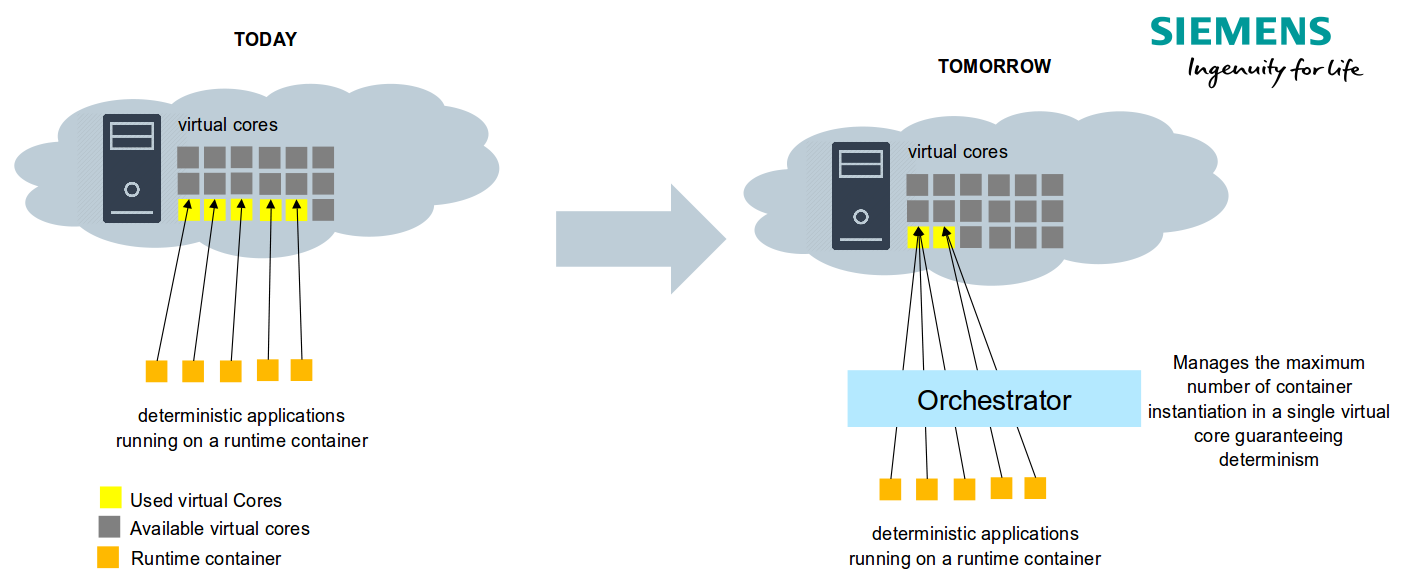
\includegraphics[width=0.8\textwidth]{plan}
	\caption{Planned resource re-allocation}
	\label{fig:plan}
\end{figure}

It is planned that this re-organization will save a major amount of resources, reducing the costs needed to operate the system while still being appropriately deterministic. To isolate the different applications from one-another, a containerized approach has been chosen beforehand. The main choices available are LXC/LXD, Docker and Balena.

LXC/LXD is the default Linux-based containerization engine and its use might not always be straight forward. This is probably one of the reasons why containerization did not take off until Docker came in. Docker is an open source project written in Go that is based on LXC/LXD technology. IT has centralized container image storage, an open API and easy to use CLI interface\footnote{see \url{docker.com} for a full list of features}. Balena on the other hand is a stripped down version of Docker, allowing to minimize the resource requirements. It uses the Docker infrastructure and has therefore a lot of its advantages while diminishing the load for the system. Balena kept most of the same configurations and parameters allowing a switch to Docker and its more advanced features at any time. For this reason Balena has been chosen as the containerization engine. Balena is an open source project hosted by resin.io.

If not further specified, sources of information for this document are:
\begin{itemize}
	\item linuxfoundation.org
	\item kernel.org
	\item docker.com
	\item resin.io
	\item balena.io
\end{itemize}

\section{System Tests and variants}

{\small\textsc{Identification of application candidates, 25-30/07/18} \bigskip}

Before selecting a specific setup, different variants of systems are tested for their real-time capabilities, maintainability and ease of setup. Candidates for this session are:

\begin{itemize}
	\item \textbf{resinOS} operating system by resin.io, designed to run containers on different architectures and hardware devices. It has Balena pre-installed and features a cloud based interface to manage the different hosts and running containers.
	\item \textbf{Ubuntu Core} an operating system for IoT devices implemented using the new snap image approach. Snap based as well as Balena based approaches are investigated on this hardware optimized image
	\item \textbf{Xenomai 3} is co-core extension for Linux based operating systems, which allows hard-real-time scheduling. Together with an interrupt patch it is suggested to be the most performing of the real-time approaches.
	\item \textbf{PREEMPT\_RT} a kernel patch for Linux-based systems which increments the achievable preemption level of the kernel. This allows for soft-real-time based performance
\end{itemize}

CoreOS has been excluded from the candidate list as it comes with a LXC/LXD image. The systems are setup in separate virtual machines and are verified for real-time scheduling properties. Installations verify the runtime behavior of containers of different types, including synthetic applications.

\subsection{resinOS by Resin.io}

{\small\textsc{Test-run resinOS, 25/07/18} \bigskip}

\textit{resinOS} is an Project-Yocto based operating system designed by ``resin.io'' for containerized running of small systems. The design also includes a cloud based monitoring system where the different configured devices connect to. The default containers supplied by resinOS are based on the lightweight general purpose Alpine Linux.

\subsubsection{Local Virtual Machine}

The resinOS operating system was primarily made to run on low resource systems, embedded devices or alike, and does thus not have a specific image for desktop/laptop or server. To run the OS in a virtual machine we download the Intel based 64 bit image for the Intel NCU from the resinOS website. \url{https://resinos.io/#downloads}

The image does not contain any additional configuration concerning network setup or ssh keys to be able to connect to the device. To configure the image, we need the CLI tool. Before installing the tool, make sure that following packages are installed:

\begin{itemize}
	
	\item \textbf{node.js 6.x} you can installa the latest version via snap using \textit{snap install node --classic --channel=x} where x can be substituted with the desired version, 8 or 10. You can also use a standard package installation. Instructions can be found at \url{https://github.com/nodesource/distributions}
	\item \textbf{npm} the node package manager is part of the node distribution. If not yet installed, install it with \textit{apt-get install npm}
	\item \textbf{rsync} versatile remote file copying tool, installable, if not already present, via \textit{apt-get install rsync}
	\item \textbf{ssh} the secure shell client is usually pre-installed on all debian based systems. If that is not the case, install it via \textit{apt-get install openssh-client}
	
\end{itemize}

Once verified that all needed software is installed, the CLI tool for resin can be added using the node package manager. Please note the need of proper privileges (sudo).

\begin{verbatim}
	npm install --global --production --unsafe-perm resin-cli
\end{verbatim}

The CLI will now allow us to configure the image as needed. For a guided configuration, and assuming the downloaded image is in \textit{~/Downloads}, type the following 

Configure the image as needed
\begin{verbatim}
	sudo resin local configure ~/Downloads/resin.img
\end{verbatim}

Manual configuration instructions and further details and documentation can be found at \url{https://resinos.io/docs/intel-nuc/gettingstarted/}.

The configured image is now ready to be deployed, but before it has to be converted to a virtual disk image in order to boot from it. Use the Virtual-Box CLI tool to execute the conversion. Once switched to the folder where the image has been downloaded, type
\begin{verbatim}
	VBoxManage convertdd resin.img resin.vdi
\end{verbatim}

Next, create new virtual machine in Virtual-Box based on ``Other Linux 64bit''. Minimum requirements are OK. Create a virtual Disk of Size of at least 4GB as main disk. 
When created, open the settings dialogue for the virtual machine. In general settings, set the parameters as in Figure \ref{fig:resingen}. Now add the boot image for resinOS in the storage menu, Figure \ref{fig:resindisk}.

\begin{figure}[t]
	\centering
	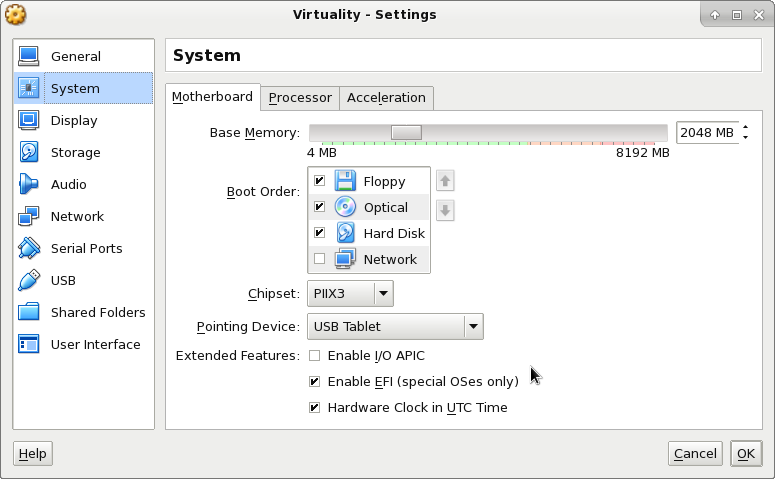
\includegraphics[width=0.8\textwidth]{resin-vbox}
	\caption{Virtualbox general settings for resinOS}
	\label{fig:resingen}
\end{figure}

\begin{figure}[t]
	\centering
	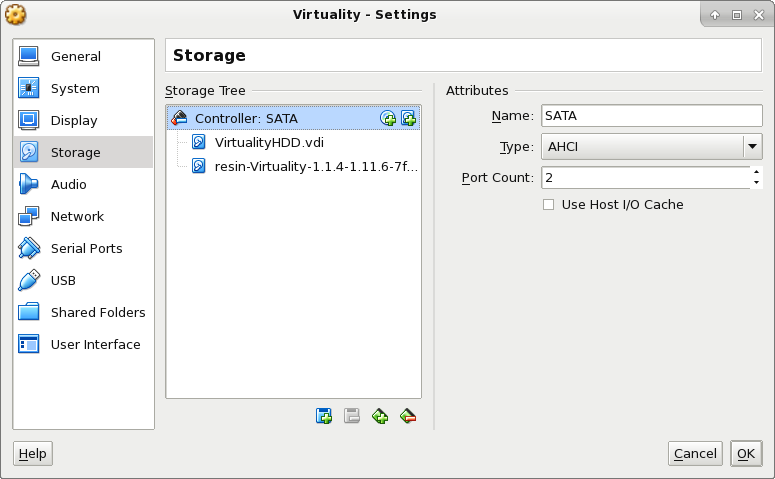
\includegraphics[width=0.8\textwidth]{resin-vbox2}
	\caption{Disk settings for resinOS}
	\label{fig:resindisk}
\end{figure}

To properly connect and download eventual containers we have to configure some forwards. In the ``Network'' menu, select advanced, then Port forward. Configure now the forward of port 8022 to 22  and 2375 to 2375 for client host 10.0.2.15 (usually).

If the virtual machine is run now, the downloaded boot image creates a new instance of resinOS on the previously created virtual drive. The new disk is populates with the settings specified in the configuration step. Once done, the system shuts down automatically and the resin boot image can be removed from the machine settings.

\subsubsection{Run a Balena container in resinOS}

As alredy discussed before, \textit{resinOS} is shipped with Balena pre-installed and the system is now ready to run any desired container. 
An example application responding to a simple web request can be set-up and tested with the following guide.

Clone the repository to a local directory with
\begin{verbatim}
	git clone https://github.com/resin-io-playground/resinos-sample
\end{verbatim}

Now enter the repository and edit ``Dockerfile''. Replace the text after FROM with \textit{resin/intel-nuc-alpine-node:slim}. Now compile and upload the container to the virtual host with

\begin{verbatim}
	sudo resin local push localhost --source .
\end{verbatim}

Setup a route from the virtual machine to the localhost, line before, from port 80 to port 8080. Browsing to localhost:8080 should now display a test page.

\subsubsection{Evaluation}

The resinOS core ships with no packager manager and is missing buildin tools. This image can therefore be patched only manually and with greater effort. This also means that it increases the maintenance effort and makes thus a resinOS based approach unpractical. In addition, the image has been tuned for small devices operation. An operation on a server infrastructure would therefore not use the maximum capabilities of the hardware constraining the system in its execution.

\subsection{Ubuntu Core}
{\small\textsc{Test-run Ubuntu core, 25/07/18} \bigskip}

Ubuntu Core is a project to bring small applications to embedded devices based on standard Ubuntu technology. The developed software is shipped in a snap and then run sandboxed in a container like environment while keeping the transparency of a traditional application. 

Snaps are standard feature of Ubuntu based distributions since 2 years now. It combines the advantages of a package manager and a virtualized container. Even though the snap itself runs on isolated resources provided through proper \texttt{cgroup} configuration, it maintains the accessibility and transparency a locally installed software would have. The running applications are practically sandboxed, having separated partitions for binaries, application specific settings, and the actual file system of the host OS. The host and the binary partitions are read-only, protecting the hosting system from eventual malicious software. In addition, the binaries are digitally signed and thus tampering with the executables is avoided. This gives the whole system the flexibility of continuous updates of an application while being independent from the host system and flavor, and without interacting with the file system of the host.
A variety of Linux flavors support snaps. In addition, snap-stores can be privately hosted, making this solution very interesting. More details can be found at \url{https://snapcraft.io/}

In this test, a setup is described and feasibility of the candidate is verified.

\subsubsection{Local Virtual machine}

Like in the previous example, the image is downloaded and ready to be used. Visit \url{https://developer.ubuntu.com/core/get-started} for an additional step-by-step guide.
First, we get and unpack the latest KVM core image (replace version numbers where appropriate):

\begin{verbatim}
	wget http://cdimage.ubuntu.com/ubuntu-core/16/stable/current/ubuntu-core-16-amd64.img.xz
	unxz ubuntu-core-16-amd64.img.xz
\end{verbatim}

Before it can be used, the image has to be converted from a raw image to a virtual drive. We convert the image again with the Virtualbox CLI tool.

\begin{verbatim}
	VBoxManage convertdd ubuntu-core-16-amd64.img ubuntu-core-16-amd64.vdi
\end{verbatim}

Now we create a new virtual machine based on Ubuntu 64bit and add the existing disk. The setup of the virtual machine is guided and therefore no additional description is given here. Standard settings are good enough. Once done, the system is ready to run.

In order to be able to connect to the new virtual machine, we need a Ubuntu one account. In the account we then specify the ssh key we are going to use to connect to the core device. The booted device will ask the email of the Ubuntu one account and downloads the ssh key. Finally to connect via ssh we have to configure some forwards. In the settings, select ``Network'', advanced, then Port forward. Configure now the forward of port 8022 to 22 for client host 10.0.2.15 (usually), the same way as described for resinOS.

For a description on how to create an ssh key, visit \url{https://confluence.atlassian.com/bitbucketserver/creating-ssh-keys-776639788.html}


\subsubsection{Evaluation}

Unfortunately, the core is stripped to minimum and thus patching for real-time capabilities is not easily possible. This means, it does not include a package manager and patching the kernel is hard as a patch command not installed.

The core used snaps for applications, thus using snaps for installations was considered. Unfortunately, even though the snap feature is native to Ubuntu, and a patched kernel could add the needed real-time properties, the binding with the hosts name and file-space hinders the use of application duplicates. This approach is thus archived for the moment.

If all other attempts are not successful enough, a conversion of the apps to snaps and proper configuration might be considered.

\subsection{Ubuntu Server 16.04.4 with Xenomai}

{\small\textsc{Testrun Xenomai, 26/07/18} \bigskip}

Xenomai is a os extension to implement POSIX real-time features to a standard kernel. Xenomai supplements it with Cobalt, a small real-time infrastructure which schedules time-critical activities independently from the main kernel logic. The interfacing with an interrupt dispatcher (I-pipe) allows to increase response time and performance and thus enables also for hard-real-time execution. Through extension with skins, also non POSIX compliant real-time software can be configured to run on a Xenomai patched system.

The main expressed concerns of this approach are setup complexity and maintainability.

\subsubsection{Local Virtual machine}
\label{sec:xenoinst}

The base-OS should be lightweight but still fully featured. Thus, an Ubuntu server flavor with minimal installation has been chosen. Download the image from the Ubuntu website \url{http://releases.ubuntu.com/16.04.4/}. The latest patches available for Xenomai/I-Pipe are based on Kernel 4.9.x and 4.14.x. Ubuntu 16.04 is the closest version with 4.4.x as the next LTS, namely Ubuntu 18.04, is shipped with Kernel 4.15.x. Thus, we select Ubuntu Server 16.04.4 as the candidate for a kernel upgrade and patch.

\begin{verbatim}
	# download image
	wget http://releases.ubuntu.com/16.04.4/ubuntu-16.04.4-desktop-amd64.iso
	# verify image hash
	curl -sfL http://releases.ubuntu.com/16.04.4/SHA256SUMS
	|	sha256sum -c 2>&1 | grep OK
\end{verbatim}

Now we create a new Ubuntu 64bit based virtual machine with a disk size of at least 20GB. Even though Ubuntu takes just a few GB, we need at least 10GB extra space for the libraries, source code and compiling process of the kernel image and header. 
The memory size for the virtual machine can be arbitrary chosen between 384 mB and $\inf$. When setting the number of assigned CPUs, consider that the more, the faster is the compiling of the new kernel. If you increase the number of CPUs, increase also the amount of RAM.
Before starting the machine, we add the Ubuntu server disk image to the cd drive of the new machine.

Now follow the guide of the installer. If asked, add only ssh server to the pre-selected packages and continue with software deployment. When installation is done, don't forget to upgrade the system to the newest packages and restart before proceeding with the kernel build. Execute:

\begin{verbatim}
	apt-get update && apt-get dist-upgrade -y
\end{verbatim}

The patching steps have all be resumed in an installer script by Pasquale Antonante. Unfortunately some steps are outdated and some configurations have changed. The script has therefore been updated and placed in the appropriate directory of this repository (ianno/real-time-containers). The install script provides downloads of the two patches, Xenomai/Cobalt and I-Pipe, the kernel, performs the patch and installs new kernel and the Balena environment.

\subsubsection{Evaluation}

Because of the way interrupt handling is implemented, allowing out-of-band interrupt handlers and thus immediate IRQ reception, Xenomai is a ideal candidate for hard-real-time constraints. The patching is bound to kernel versions, thus the progress depends on the patch development of I-Pipe. 
The scheduling of the real-time tasks is based on the co-kernel and is thus easier to modify and change, a promising approach.
Currently the kernel patch is stuck at version 4.14.4 (the latest kernel shipped with Ubuntu 16.04 LTS is 4.15.0-29, the latest stable 4.17.11). This could be a sign of an abandoned project. Before continuing with this implementation line, a proper investigation of the project status and agenda must be performed.

\subsection{Ubuntu Server 16.04.4 with patch RT}

{\small\textsc{Testrun Preempt-RT, 27/07/18} \bigskip}

PREEMPT\_RT is a real-time kernel project maintained by the Linux foundation. 
The main aim of the PREEMPT\_RT patch is to minimize the amount of kernel code that is non-preemptible. Therefore several substitutions and new mechanisms are implemented.
In the last years there where some major improvements in PREEMPT-RT. A paper of Fayyad-Kazan \textit{et al.} shows improvement on kernel versions v2.6.33 versus v3.6.6, a total improvement of 35\% \cite{Fayyad-Kazanetal2014}. In order to keep performances and results comparable, the same Ubuntu image will be used for patching.

\subsubsection{Local Virtual machine}

The same conditions as in the previous example apply. Download the image from the Ubuntu website \url{http://releases.ubuntu.com/16.04.4/}, if not already done. Also here the latest patch available for Ubuntu is based on Kernel 4.9.x. Ubuntu 16.04 is again the closest version with 4.4.x and thus the candidate for a kernel upgrade. See section \ref{sec:xenoinst}.

The patching steps have all be resumed in an installer script similar to the previous. The install script provides downloads of the patch and the kernel, performs the patch and installs new kernel and the Balena environment.

%downloaded patched kernel from kernel.org
%make menuconfig
%-> (needs libncurses5 libncurses5-dev)
%remove cpu-freq and cpu idle (needs PM cpu deactivation first)

For further guides on how to compile and install a kernel, visit \url{ https://medium.freecodecamp.org/building-and-installing-the-latest-linux-kernel-from-source-6d8df5345980}

\subsubsection{Evaluation}

The Preempt-RT requires a dedicated patch and recompiling of the kernel to support soft-real-time properties. The additional slicing preformed to the kernel tasks allows faster preemption and a better control of the CPU scheduling. Compared to the previous example, the handling of interrupt flow can not be controlled to the same extend reaching thus a lower level of real-time feasibility. Anyway, lately the project has made remarkable progress.
Its mainline development is following kernel distribution at a fast pace, indicating that the project is strongly followed and has a valuable community backup. This makes this solution a major candidate for further investigation.
To exploit its full potential, an Ubuntu 18.04 LTS kernel patching as a future step is taken into consideration.

\section{Tests of system}

{\small\textsc{Testrun and comparison of systems, 30/07/18} \bigskip}

Some small cyclic execution tests are performed to verify default availability of real-time sheduling and the timing behavior of the scheduler.

\subsection{rt-tests}

the rt-tests suite includes a list of small tool binaries which may be used to test properties of real-time systems. The most prominent are \textit{cyclictest} and \textit{hackbench}. To install the software we may use one of the two approaches:

1) We use Xenomai, thus there is a tool package ready and available

\begin{verbatim}
	apt-get install xenomai-system-tools
\end{verbatim}

2) We use another real-time approach and compile the binaries from the source code.
For this approach we need first some additional packages. Get them with:

\begin{verbatim}
	sudo apt-get install build-essential libnuma-dev
\end{verbatim}

Now proceed with the installation. Download the git repository and compile the source.

\begin{verbatim}
	git clone git://git.kernel.org/pub/scm/utils/rt-tests/rt-tests.git
	cd rt-tests
	git checkout stable/v1.0
	make all
	make install
\end{verbatim}

The last step is optional. The binaries can now be run (within the directory) to perform the different tests. An example of a test, as recommended on Kernel.org is: 

\begin{verbatim}
	cyclictest -t 50 -n -d 86400 -l 100000 -a -p 99
\end{verbatim}

The code in the example creates fifty tasks with priority 99 (maximum) an interval of 1000 $\mu s$ and a task delay of 86400 $\mu s$ and using a clock-based nanosecond timer. 
As an example, we compared the results between virtual machines of the different kinds we have set up by now. There is a difference between normal and patched images, but the actual values are for now far from ideal. At the moment, as the host is not real-time capable, the delays also depend on the scheduling of the host which sets up the virtual machine. 

\subsection{stress}

In order to verify behaviour also under stress we use the tool \textit{stress}. The installation can be performed by downloading and compiling the source code. Further information can be found at \url{http://people.seas.harvard.edu/~apw/stress/}.

\begin{verbatim}
	#download and extract
	curl -sfL http://people.seas.harvard.edu/~apw/stress/stress-1.0.4.tar.gz | tar xvz
	# compile and install
	cd stress-1.0.4
	./configure
	sudo make install
\end{verbatim}

An example execution can be performed via the command:

\begin{verbatim}
	stress -d 3 --hdd-bytes 20M -c 3 -i 3 -m 3 --vm-bytes 15M
\end{verbatim}

\subsection{Other testing tools}

A list of other tools that might be helpful:

\begin{itemize}
	\item \textbf{htop} a colored memory view to analyse memory use of single processes
	\item \textbf{iftop} interface monitor to view actual network traffic
	\item \textbf{iotop} generic i/o monitor
\end{itemize}

\section{Additional fixes}
{\small\textsc{Configuration test, 31/07/18} \bigskip}

Balena, even though installed via script, appears not properly configured. It does not run at startup and there is no typical dedicated group in order to ease and limit access to the engine.
Therefore groups and systemd configuration files to manage these must be added manually. Use the docker reference manual to provide for this. The manual can be found at \url{https://docs.docker.com/reference/}. The balena daemon is started via the command \textit{balenad}.

\begin{figure}[t]
	\centering
	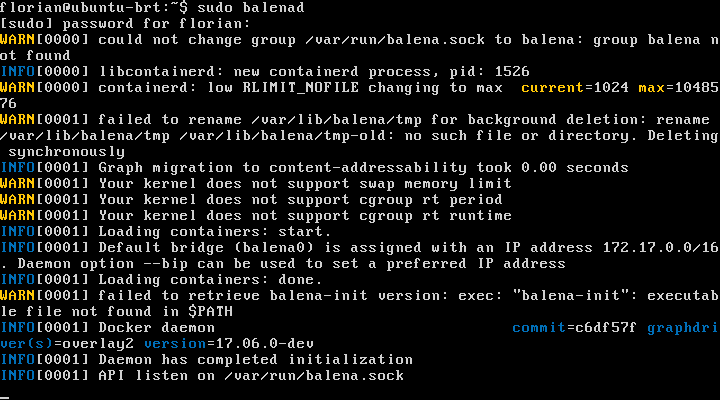
\includegraphics[width=0.8\textwidth]{balena-err}
	\caption{Error messages displayed by Balena at first run}
	\label{fig:balenad}
\end{figure}

An additional not clear thing is the missing of the \texttt{balena-init} file, see \ref{fig:balenad}. Comparing the installation to the standard resinOS shipping we can see that the latter has the missing file and they have the same version number, but also, that the main binary is different in size. It is unclear what this might mean. The init binary is intended to initialize a newly created container in order to remove al the orphanage resources and prepare the new container for a clean run. According to th docker reference manual, \url{https://docs.docker.com/engine/reference/run/}, the init binary is obtained via tini, thus can be safely pulled from there. The git repository can be found at \url{https://github.com/krallin/tini/tree/v0.18.0}.

In the image also other warnings can be found. In particular we can identify two groups of warnings:

\begin{itemize}
	\item \textit{WARN[0001] Your kernel does not support swap memory limit}

	\item \textit{WARN[0001] Your kernel does not support cgroup rt period} and \textit{WARN[0001] Your kernel does not support cgroup rt runtime} 
\end{itemize}

The former is due to the fact that memory swap support has not been enabled ad kernel built time. 
The configuration setting to be enabled is \texttt{\#CONFIG\_MEMCG\_SWAP\_ENABLED}. As a temporary fix we can enable the settings at boot-time. 
To do this we edit \texttt{/etc/default/grub} and set 
\texttt{GRUB\_CMDLINE\_LINUX\_DEFAULT} to \texttt{"cgroup\_enable=memory swapaccount=1"}

The latter of the two warning groups is also due to a configuration setting of the kernel. They concern the real-time run-time control of single cgroups. This is a feature which is needed/used in containers when we want to control the single containers' maximum cpu execution slice, see \url{https://docs.docker.com/config/containers/resource_constraints/}. 
In fact, if we try to set some of the real-time settings on our running balena instance we get the following error message: \textit{balena: Error response from daemon: Your kernel does not support cgroup cpu real-time runtime.}.
The required setting can be enabled at kernel compilation time via the \texttt{CONFIG\_RT\_CGROUP} flag. 
Unfortunately the flag can not be enabled for the PREEMPT\_RT version of the virtual machine. Due to some temporary compatibility constraints, the simultaneous operation of the \texttt{CONFIG\_PREEMPT\_FULL} flag, necessary for the ability of full kernel preemption, and the CGroup flag has been disabled. Details can be found at \url{https://wiki.linuxfoundation.org/realtime/documentation/known_limitations#disabled-config_-options}.

Finally, I found a script that could do the verifications for you. If you would like to test your system for parameter and capability compliance, the docker comunity has developed a configuration testing script. The test can be run via these inputs:

\begin{verbatim}
	wget https://raw.githubusercontent.com/dotcloud/docker/master/contrib/check-config.sh
	chmod =x check-config.sh
	./check-config.sh
\end{verbatim}

The run of the script confirms that the Xenomai version of the image, after all reconfiguration and recompilation, has the correct settings to operate the container engine properly.

\section{Virtualization sustainability tests}

{\small\textsc{Testrun Containers \& CPU pinning, 01/08 - 03/08/18} \bigskip}

% AWS ? virtual machine test resoure pinning in vbox -> pin local host? balance share.

In this section we verify the real-time latencies in different settings and how the applications behave inside a container. In order to do this, a variety of system configurations are performed and capabilities verified. The list of all capabilities can be viewed on every Linux based system by typing \texttt{man 7 capabilities} into a shell.

During some additional research on Balena and its relation to Docker, the source code of Balena actually revealed that the use and parameters for the compose program, namely \texttt{docker-compose}, is available to run also on a Balena based engine. In addition, in the documentation of resinOS, \url{https://docs.resin.io}, the instructions specify to install docker-compose on a remote system and operate the containers via remote.
\texttt{docker-compose} is a tool written in python which allows to configure and connect multiple containers using a single json file even from a remote machine, a welcome feature for our project.
Anyway, by the source code of Balena we can tell that not all the tags are supported. This is particularly valid for the `Deploy' section.

More detail on the different operations taken in this section and on the why those are performed, can be found at \url{http://linuxrealtime.org/index.php/Basic_Linux_from_a_Real-Time_Perspective}.

\subsection{Preparing steps}

In preparation for the upcoming tests we need to install docker-compose and configure the proper cpu-isolation for the virutal machine.
The instructions can be found in the reference of docker, see  \url{https://docs.docker.com/compose/install/}. 
On debian systems this can be done simply via 

\begin{verbatim}
	apt-get install docker-compose
\end{verbatim}

During these tests, the virtual machine is set to 3 cpus, and the cpu afinity of the task on the host is set to 7 (cpu 0,1,2). This will allow to avoid task switching and further separate RT tasks (cpu 0-1) from nRT tasks (cpu 2) inside the virtual machine
In the settings of the virtual machine we set the CPUs to 3 and we start the virtual machine.  Open a process monitor, e.g. the system monitor, and get the pid of the running virtual host. Open a console and use the following command-line (\url{https://forums.virtualbox.org/viewtopic.php?p=45847}):

\begin{verbatim}
	taskset -p 7 <read-pid>
\end{verbatim} 

The virtual machine is now running confined to CPUs 1, 2 and 3.

\subsection{CPU isolation and partitioning tests}

Let us try to start with some first measurements. We will run the tool cyclictest in different combinations, with and without stress on the CPU.

\subsubsection{no load, 3 cpus}

\noindent Command : \textit{cyclictest -n -m -p 99 -l 100000}

\noindent Results :

\noindent \texttt{T: 0 ( 1489) P:99 I:1000 C: 109551 Min:      0 Act: 4894 Avg: 1370 Max:  4914811}

\subsubsection{load 3cpus}

\noindent Command : \textit{stress -d 3 --hdd-bytes 20M -c 3 -i 3 -m 3 --vm-bytes 15M \& cyclictest -n -m -p 99 -l 100000;}

\noindent Results :

\noindent \texttt{T: 0 ( 1514) P:99 I:1000 C: 100000 Min:      2 Act:   88 Avg:  358 Max:   23924}

\subsubsection{no load, 3 cpus, isolation}

\textbf{CGroups} is a standard Linux feature used for resource partitioning and CPU pinning (affinity selection). It is one of the techniques also used by Balena \& Co. to isolate the containers from the host. It is a technique that might be used in combination with previous systems in order to increase the real-time properties. The tool \textit{cpuset} allows to perform a lot of the manual steps needed in an easier manner. 

Thus, in oder to give the virtual machine proper computing power, isolate it from the host processes, and to allow isolation of the real-time tasks from non real-time processes, we will now set up cpu isolation for the host CPU. A two core machine will usually have four vCPUs, meaning two cores and two threads per core which equals 4. Thus we will assign vCPUs 0-2 to the virtual guest and CPU 3 for the host system.

First we need to install the \texttt{cpuset} utility.This can be done via:

\begin{verbatim}
	apt-get install cpuset
\end{verbatim}

Next we set-up the CPU-isolation. Open a process monitor, e.g. the system monitor, and get the pid of the running virtual host. Open a shell and change to root (or use sudo):

\begin{verbatim}
	sudo cset shield -c 0-2 -k on --shield
	sudo cset shield --shield --threads --pid <read-pid>
\end{verbatim}

The virtual machine and all depending tasks are now moved to a separate control group which has exclusive access to the vCPUs 0 to 2. All tasks of the host, where possible, have been moved to vCPU 3 (verify with \texttt{cset set -l --shield} and \texttt{cset set -l --unshield}). In Figure \ref{fig:test-cpu} the effect on the host of cpu-isolation is shown.

\begin{figure}[t]
	\centering
	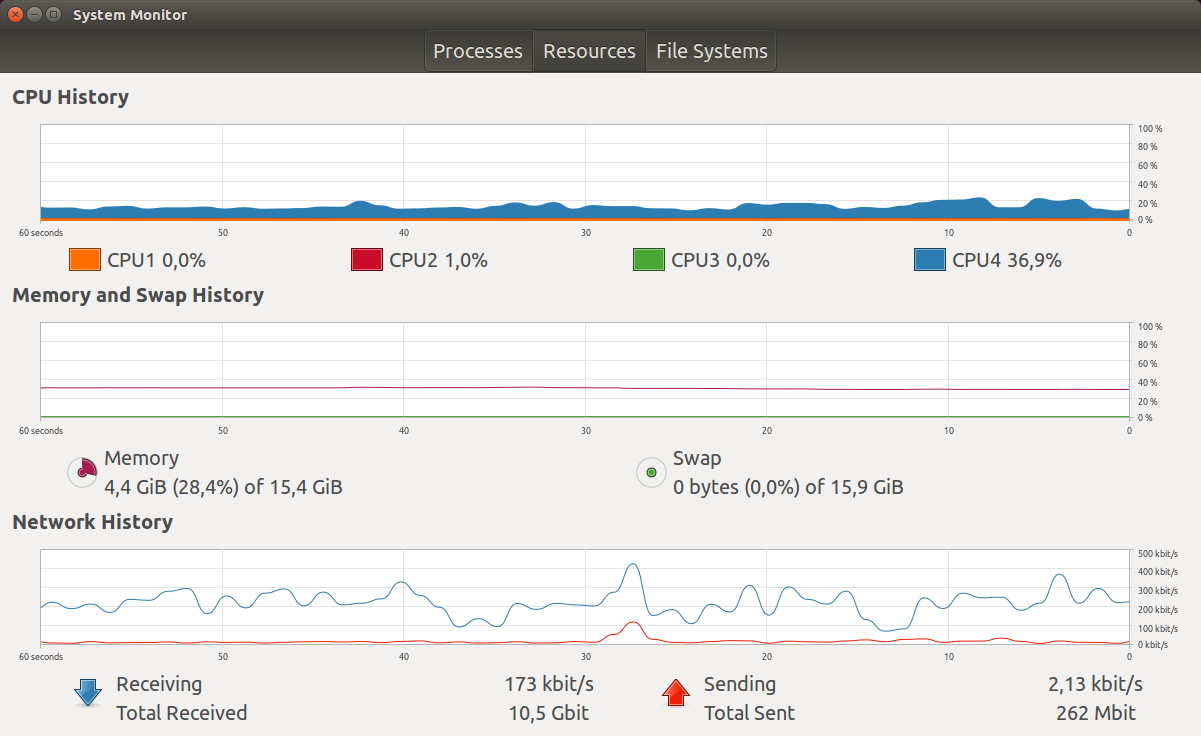
\includegraphics[width=0.8\textwidth]{test-cpu}
	\caption{System monitor showing the isolated virtual machine (idle) and the loaded host vCPU}
	\label{fig:test-cpu}
\end{figure}

%TODO:---verify again ths> ,7 secs seems much

\noindent Command : \textit{cyclictest -n -m -p 99 -l 100000}

\noindent Results :

\noindent \texttt{T: 0 ( 1431) P:99 I:1000 C: 100000 Min:      0 Act:  263 Avg: 1319 Max:  7618166}

\subsubsection{load 3cpus, isolation}

In this second test we put again the virtual machine under load. The system's CPU load can be seen in Figure \ref{fig:test-cpuload}. It is as expected balanced on the three vCPUs dedicated to the virtual guest.

\noindent Command : \textit{stress -d 3 --hdd-bytes 20M -c 3 -i 3 -m 3 --vm-bytes 15M \& cyclictest -n -m -p 99 -l 100000;}

\noindent Results : 

\noindent \texttt{T: 0 ( 1358) P:99 I:1000 C: 100000 Min:      0 Act:   49 Avg:  337 Max:   233955}


\begin{figure}[t]
	\centering
	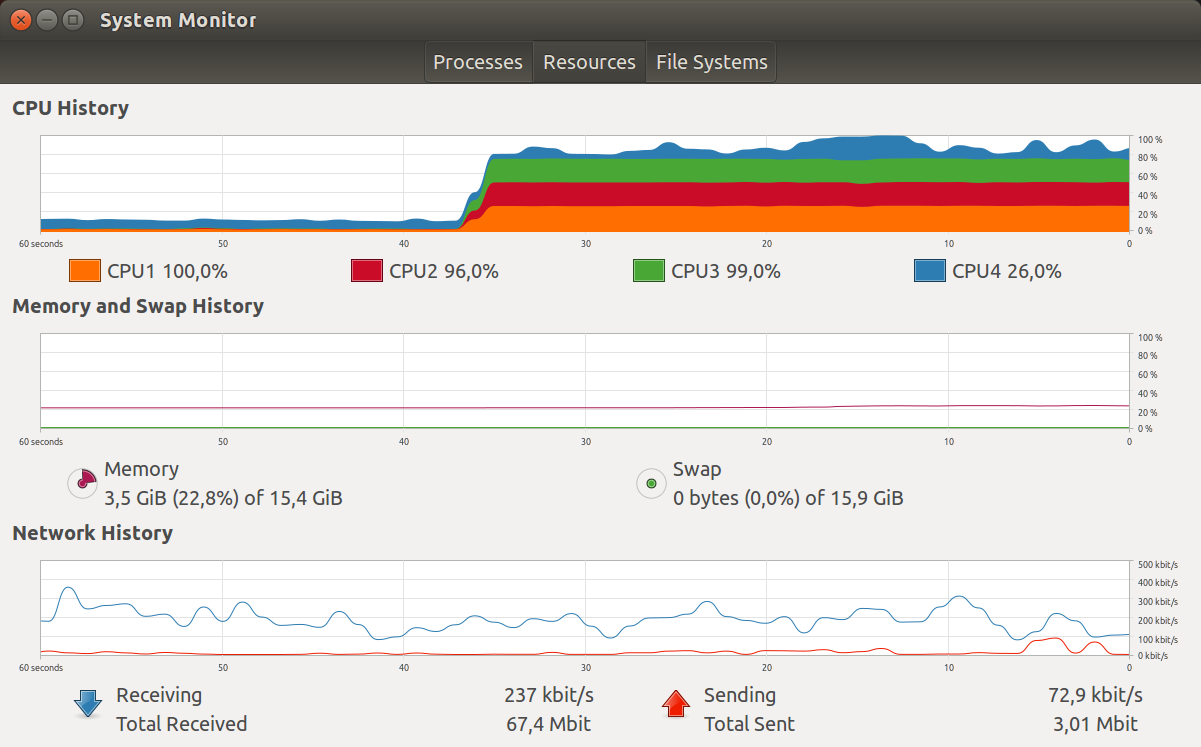
\includegraphics[width=0.8\textwidth]{test-cpuload}
	\caption{System monitor showing the same isolated virtual machine under load}
	\label{fig:test-cpuload}
\end{figure}

\subsubsection{no load 3cpus, isolation, no load balancer}

Even though the threads of the virtual machine are confined on the tree cpus, the load balancer of the Complete Fair Scheduler (CFS) is still active. We test now what happens when we deactivate the scheduler:

\begin{verbatim}
	#Removing load balancer
	echo 0 > /sys/fs/cgroup/cpuset/cpuset.sched_load_balance
	echo 0 > /sys/fs/cgroup/cpuset/user/cpuset.sched_load_balance
	echo 1 > /sys/fs/cgroup/cpuset/system/cpuset.sched_load_balance
\end{verbatim}
%\bigskip

\noindent Command : \textit{cyclictest -n -m -p 99 -l 100000}

\noindent Results :

\noindent  \texttt{T: 0 ( 1452) P:99 I:1000 C: 100000 Min:      0 Act: 2815 Avg: 2183 Max:  8679855}

\subsubsection{no load 3cpus, isolation, irq affinity}

For now only the tasks, user or system, have been moved from their original CPU to vCPU 3. Interrupts on a multicore system can be triggered on every active core and handled by the the specific routine. To isolate further the virtual machine and move the IRQs only to vCPU 3 we can use the following command: 

\begin{verbatim}
	# move irq affinity to Cpu 3
	for file in /proc/irq/*; do   echo 3 > \$file/smp_affinity; done
\end{verbatim}

The new test/results is then as follows:

\noindent Command : \textit{cyclictest -n -m -p 99 -l 100000}

\noindent Results :

\noindent \texttt{T: 0 ( 1456) P:99 I:1000 C: 100000 Min:      0 Act:  198 Avg: 1693 Max:  9862777}

\subsubsection{Cpu-isolation guest, host no load balancer \& irq affinity }

1CPU fully to RT, 1 Thread to nRT, 1 Thread to host

set cpu affinity isolating rt from system in guest
\bigskip

\noindent Command : 

\begin{verbatim}
	# run shielding
	cset shield -c 0-1 -k on --shield
	# start test
	cyclictest -n -m -p 99 -l 100000
	# enable shield on test pid
	cset shield --shield --threads --pid <cycletest pid>
\end{verbatim}

\noindent Results :

\noindent \texttt{T: 0 ( 1664) P:99 I:1000 C: 100000 Min:      0 Act: 3037 Avg: 1913 Max:  2011888}

\subsubsection{Conclusions isolation Host}

We have seen in this first validation results that a VirtualBox task can be pinned to a certain CPU-set. The results of the reaction times are varying with unclear reasons. One main reason could be that the last vCPU is not actually a separate core but only one of the two threads of the HyperThreading instance of the physical core two. Thus it is possible that the increase in the max latency is due to the interrupt overload on the shared physical CPU, influencing thus directly the maximum performance and average latency of the real-time tasks.

The most fluid setting for the isolation of the guest system is thus simple cpu shielding (isolation) done with cset. Therefore, for the rest of the document, we assume a test machine where 3 vCPUs (cores) = 1 cpu HT + 1 Thread of CPU2, have been assigned to the virtual machine.

\subsubsection{Cpu-isolation guest, host back to simple isolation}

after puttng load balance and irq settings of host back to normal

\noindent Command : \textit{cyclictest -n -m -p 99 -l 100000}

\noindent Results :

\noindent \texttt{T: 0 ( 1695) P:99 I:1000 C: 100000 Min:      0 Act:   73 Avg:  148 Max:    4773}

\subsubsection{Cpu-isolation guest, set irq affinity \& no load balancer}

setting irq affinity to 2
and load balancing to off like for host

\noindent Command : \textit{cyclictest -n -m -p 99 -l 100000}

\noindent Results :

\noindent \texttt{T: 0 ( 1698) P:99 I:1000 C: 100000 Min:      0 Act:   62 Avg:  186 Max:    4850}

\subsubsection{Cpu-isolation guest, test multiple}

--- going up wo shild?

\noindent Command : \textit{cyclictest -t2 -n -m -p 99 -l 100000}

\noindent Results :

\noindent  
\texttt{T: 0 ( 1711) P:99 I:1000 C:  34925 Min:      2 Act: 2605 Avg:  932 Max:    9958}
\noindent
\texttt{T: 1 ( 1712) P:99 I:1500 C:  26368 Min:      1 Act: 2121 Avg: 1059 Max:   10389}


\subsubsection{Counterproof isolation Host}

unshielded host -> delay tasks go to the sky again!
if we remove shield on host, we get back to the first result again.

\subsection{improve rt properties}

http://linuxrealtime.org/index.php/Improving_the_Real-Time_Properties


%TODO: CONFIG_NO_HZ_FULL ? effect on kernel?

To achieve full dynamic ticks on a CPU, there are some requirements on the application being run on this CPU. First of all, it must not run more than one thread on each CPU. It must also not use any POSIX timers, directly or indirectly. This usually excludes any kernel calls that will access the network, but also excludes a number of other kernel calls. Keeping the kernel calls to a minimum will maximize the likelihood of achieving full dynamic ticks.

The application must utilize the CPU partitioning described in previous section, which is done by writing the application thread's PID into the file /sys/fs/cgroup/cpuset/rt/cpuset.tasks (assuming the real-time partition is called "rt"). After this, the shell command taskset can be used to bind the task to a specific CPU in the "rt" partition. Binding can also be done by the application itself using the sched_setaffinity() function defined in sched.h.


AWS vCPU scheduler description
https://wiki.xenproject.org/wiki/Xen_Project_Schedulers



\subsection{Tests balena container}

Docker application running as a real-time task. creation of a dummy task, mabye through stress application in container? it is real-time capable

start balenad with host listen option, by default it listens to localhost, meaning 0.0.0.0 127.0.0.1

balenad -H 10.0.2.15:2375 to add listen to host, default is localhost 0.0.0.0 loop interface?

add port forward to 2375 port


------
tests with rt runtime..
limit of runtime for docker must be <= the max amount specified
/sys/fs/cgroup/cpu/cpu.rt\_runtime\_us 

whereas docker settings are specified 
/sys/fs/cgroup/cpu,cpuacct/docker/cpu.rt\_runtime\_us
or via command line. then every container can range in this limit

same is true for the period parameters (docker and general)


\section{Final considerations, Meeting decisions and updated remarks}

{\small\textsc{Study of further docs and sources, 06/08 - 07/08/18} \bigskip}

Docker chosen as a main visualization platform. Kubernetes as management tool for the virtualized machine. Therefore we use a C5 instance with at least 4 cores and in addition a generic instance with a Kubernetes monitoring system.

\url{https://en.wikipedia.org/wiki/SCHED_DEADLINE}

``Since kernel 4.13, SCHED\_DEADLINE completed CBS with the Greedy Reclamation of Unused Bandwidth (GRUB) algorithm.[35] The support has been developed by ReTiS Lab with the collaboration of Evidence Srl.''


https://www.kernel.org/doc/Documentation/scheduler/sched-rt-group.txt
https://www.kernel.org/doc/Documentation/scheduler/sched-deadline.txt


https://github.com/scheduler-tools !!!


\section{Meetings}

\begin{table}[h]
	\centering
	\caption{List of meetings during the stay at UC Berkeley}
	
	\begin{tabular}{l p{5cm} p{5cm}}
	Date & Participants & Topics \\
	\hline
	26/07/18 & Martin Sehr, Ines Ugalde Diaz, Antonio Iannopollo, Florian Hofer & Project setup, generic requirements, questions for BU\\
	31/07/18 & Martin Sehr, Ines Ugalde Diaz, Florian Hofer & Progress of testing, Dummy testing approach\\
	07/08/18 & Martin Sehr, Ines Ugalde Diaz, Antonio Iannopollo, Florian Hofer & Switch to Docker and Kubernetes in Ubuntu Server 18.04\\
	10/08/18 & Martin Sehr, Ines Ugalde Diaz, Florian Hofer & ``Suspended''\\
	\hline
	\end{tabular}
	
	\label{tab:meeting}
\end{table}

\bibliographystyle{IEEEtran}
\bibliography{IEEEabrv,bibliography}

\end{document}


% Fri Non slide 



